\documentclass{beamer}
\usepackage[utf8]{inputenc}
\usepackage[english]{babel}
\usepackage{helvet}
\usepackage[T1]{fontenc}
\usepackage{textcomp}
\usepackage[inline]{asymptote}
\usepackage{slide_helper}
\usepackage{tikz}
\usetikzlibrary{shapes.geometric, arrows}
\usepackage{pgfplots}
\pgfplotsset{compat=1.5} 
\usepgfplotslibrary{statistics}
\usetikzlibrary{external}
\tikzexternalize%

\title[MA205 - Section 2.1]{Examining Numerical Data}

\begin{document}
\begin{frame}
\titlepage
\end{frame}

\begin{frame}
\begin{example}
Let us consider a scatterplot of borrowers total income and the loan amount from the \texttt{loan50} data set.

\only<1| handout:0>{
\begin{center}
\begin{tikzpicture}
\tikzstyle{every pin}=[
fill=white,
draw=black,
font=\tiny,
]
\pgfkeys{/pgf/number format/.cd,
fixed,
precision=999,
set thousands separator={},
1000 sep in fractionals=false,
}
\begin{axis}[
clip mode=individual,
clip marker paths=true,
width=10cm,
height=5cm,
xlabel={Total Income},
ylabel={Loan Amount},
grid=major,
%ymajorgrids=true,
%xmajorgrids=true,
%enlarge x limits=false,
%enlarge y limits=false,
%xticklabel style={/pgf/number format/.cd,fixed,precision=0},
xticklabel=\$\pgfmathprintnumber{\tick}k,,
yticklabel=\$\pgfmathprintnumber{\tick}k,,
xtick={0, 50000, 100000, 150000, 200000, 250000, 300000},
ytick={0, 10000, 20000, 30000, 40000},
scaled x ticks=base 10:-3,
xtick scale label code/.code={},
scaled y ticks=base 10:-3,
ytick scale label code/.code={},
ymin=-5,
ymax=35000,
xmin=-5,
xmax=325000,
scatter/use mapped color={
%draw=mapped color,
fill=black,
},
]
\addplot [scatter, only marks, blue!50!black, scatter src=y, mark size=0.8pt] 
table [y=loan_amount, x=total_income, col sep=comma] {loan50.csv};
\end{axis}
\end{tikzpicture}
\end{center}
}
\only<2->{
\begin{center}
\begin{tikzpicture}
\tikzstyle{every pin}=[
fill=white,
draw=black,
font=\tiny,
]
\pgfkeys{/pgf/number format/.cd,
fixed,
precision=999,
set thousands separator={},
1000 sep in fractionals=false,
}
\begin{axis}[
clip mode=individual,
clip marker paths=true,
width=10cm,
height=5cm,
xlabel={Total Income},
ylabel={Loan Amount},
grid=major,
%ymajorgrids=true,
%xmajorgrids=true,
%enlarge x limits=false,
%enlarge y limits=false,
%xticklabel style={/pgf/number format/.cd,fixed,precision=0},
xticklabel=\$\pgfmathprintnumber{\tick}k,,
yticklabel=\$\pgfmathprintnumber{\tick}k,,
xtick={0, 50000, 100000, 150000, 200000, 250000, 300000},
ytick={0, 10000, 20000, 30000, 40000},
scaled x ticks=base 10:-3,
xtick scale label code/.code={},
scaled y ticks=base 10:-3,
ytick scale label code/.code={},
ymin=-5,
ymax=35000,
xmin=-5,
xmax=325000,
scatter/use mapped color={
%draw=mapped color,
fill=black,
},
]
\addplot [scatter, only marks, red, scatter src=y, mark size=1.0pt,, scatter/use mapped color={fill=red,}]
table [y=loan_amount, x=total_income, col sep=comma, x expr={\thisrow{total_income} / (\thisrow{total_income} <= 100000)}] {loan50.csv};
\addplot [scatter, only marks, blue!50!black, scatter src=y, mark size=0.8pt]
table [y=loan_amount, x=total_income, col sep=comma, x expr={\thisrow{total_income} / (\thisrow{total_income} > 100000)}] {loan50.csv};
\addplot [mark size=0pt, red, line width=0.5pt] coordinates {(100000,0) (100000,35000)};
\end{axis}
\end{tikzpicture}
\end{center}
}\pause

We can see that the many of borrowers earn \$100,000 a year or less.
\end{example}
\end{frame}

\begin{frame}
\begin{example}
Let us consider a scatterplot of borrowers total income and the loan amount from the \texttt{loan50} data set.

\only<1| handout:0>{
\begin{center}
\begin{tikzpicture}
\tikzstyle{every pin}=[
fill=white,
draw=black,
font=\tiny,
]
\pgfkeys{/pgf/number format/.cd,
fixed,
precision=999,
set thousands separator={},
1000 sep in fractionals=false,
}
\begin{axis}[
clip mode=individual,
clip marker paths=true,
width=10cm,
height=5cm,
xlabel={Poverty Rate},
ylabel={Median Household Income},
grid=major,
%ymajorgrids=true,
%xmajorgrids=true,
%enlarge x limits=false,
%enlarge y limits=false,
%xticklabel style={/pgf/number format/.cd,fixed,precision=0},
xticklabel=\pgfmathprintnumber{\tick}\%,
yticklabel=\$\pgfmathprintnumber{\tick}k,
xtick={0, 10, 20, 30, 40, 50},
ytick={0, 20000, 40000, 60000, 80000, 100000, 120000},
%scaled x ticks=base 10:-3,
%xtick scale label code/.code={},
scaled y ticks=base 10:-3,
ytick scale label code/.code={},
ymin=-5,
ymax=125000,
xmin=-5,
xmax=60,
scatter/use mapped color={
%draw=mapped color,
fill=black,
},
]
\addplot [scatter, only marks, blue!50!black, scatter src=y, mark size=0.3pt] 
table [y=median_hh_income, x=poverty, col sep=comma,ignore chars={N,A}] {county.csv};
\end{axis}
\end{tikzpicture}
\end{center}
}
\only<2->{
\begin{center}
\begin{tikzpicture}
\tikzstyle{every pin}=[
fill=white,
draw=black,
font=\tiny,
]
\pgfkeys{/pgf/number format/.cd,
fixed,
precision=999,
set thousands separator={},
1000 sep in fractionals=false,
}
\begin{axis}[
clip mode=individual,
clip marker paths=true,
width=10cm,
height=5cm,
xlabel={Poverty Rate},
ylabel={Median Household Income},
grid=major,
%ymajorgrids=true,
%xmajorgrids=true,
%enlarge x limits=false,
%enlarge y limits=false,
%xticklabel style={/pgf/number format/.cd,fixed,precision=0},
xticklabel=\pgfmathprintnumber{\tick}\%,
yticklabel=\$\pgfmathprintnumber{\tick}k,
xtick={0, 10, 20, 30, 40, 50},
ytick={0, 20000, 40000, 60000, 80000, 100000, 120000},
%scaled x ticks=base 10:-3,
%xtick scale label code/.code={},
scaled y ticks=base 10:-3,
ytick scale label code/.code={},
ymin=-5,
ymax=125000,
xmin=-5,
xmax=60,
scatter/use mapped color={
%draw=mapped color,
fill=black,
},
]
\addplot [scatter, only marks, blue!50!black, scatter src=y, mark size=0.3pt] 
table [y=median_hh_income, x=poverty, col sep=comma,ignore chars={N,A}] {county.csv};
\addplot [domain=0:50,red, line width=1pt] {84923*e^(-0.0342*x)};
\end{axis}
\end{tikzpicture}
\end{center}
}\pause
It is clear there is a \textbf{nonlinear} association between the median household income and the poverty rate.
\end{example}
\end{frame}

\begin{frame}
\begin{definition}
A \textbf{dot plot} is a one-variable scatterplot. Each data value is plotted as a point above a horizontal scale of values. Dots representing equal values are stacked.
\end{definition}\pause

\begin{example}
\begin{center}
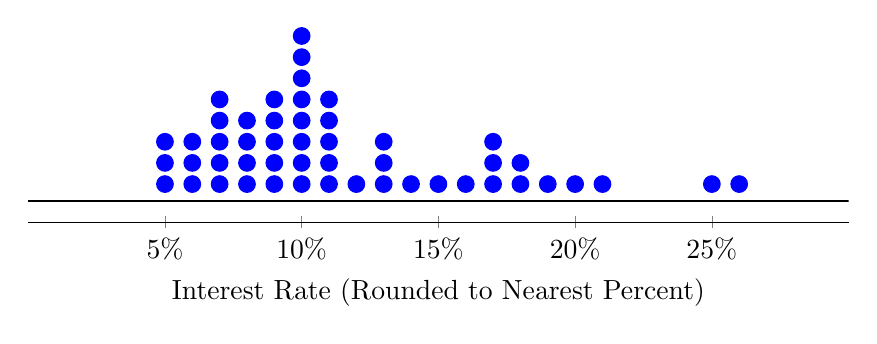
\begin{tikzpicture}
\pgfplotsset{ every non boxed x axis/.append style={x axis line style=-},
     every non boxed y axis/.append style={y axis line style=-}}
\begin{axis}[
width=12cm,
height=4cm,
xlabel={Interest Rate (Rounded to Nearest Percent)},
ylabel={},
yticklabels={},
axis y line=none,
axis x line=bottom,
xticklabel=\pgfmathprintnumber{\tick}\%,
xtick={5,10,15,20,25},
ymin=0,
ymax=9,
xmin=0,
xmax=30,
scatter/use mapped color={
 %draw=mapped color,
 fill=blue,
},
]
\addplot [domain=0:30]  {1};
\addplot[scatter, only marks, blue, scatter src=y, mark size=3pt]
coordinates
{
(11, 1.8)
(11, 2.8)
(11, 3.8)
(11, 4.8)
(11, 5.8)
(10, 1.8)
(10, 2.8)
(10, 3.8)
(10, 4.8)
(10, 5.8)
(10, 6.8)
(10, 7.8)
(10, 8.8)
(26, 1.8)
(9, 1.8)
(9, 2.8)
(9, 3.8)
(9, 4.8)
(9, 5.8)
(17, 1.8)
(17, 2.8)
(17, 3.8)
(6, 1.8)
(6, 2.8)
(6, 3.8)
(8, 1.8)
(8, 2.8)
(8, 3.8)
(8, 4.8)
(13, 1.8)
(13, 2.8)
(13, 3.8)
(5, 1.8)
(5, 2.8)
(5, 3.8)
(7, 1.8)
(7, 2.8)
(7, 3.8)
(7, 4.8)
(7, 5.8)
(25, 1.8)
(18, 1.8)
(18, 2.8)
(19, 1.8)
(14, 1.8)
(20, 1.8)
(15, 1.8)
(12, 1.8)
(16, 1.8)
(21, 1.8)
};
\end{axis}
\end{tikzpicture}
\end{center}
\end{example}\pause

\begin{note}
Dot plots work best with integer data. It is common to round decimals before building a dot plot.
\end{note}
\end{frame}

\begin{frame}
\begin{definition}
A \textbf{parameter} is a numerical measurement describing some characteristic of a population.
\end{definition}\pause
\begin{definition}
A \textbf{statistic} is a numerical measurement describing some characteristic of a sample.
\end{definition}\pause
\begin{note}
Parameter and population both start with a \textquote{P.}\\Statistic and sample both start with a \textquote{S.}
\end{note}
\end{frame}

\begin{frame}
\begin{definition}
A \textbf{measure of center} is a value at the center or middle of a data set.
\end{definition}\pause

\begin{definition}
The \textbf{mean} of a set of data is the measure of center found by adding all the data values and dividing by the total number of data values.
\end{definition}\pause

\begin{note}
The mean is also known as the \textbf{average}.
\end{note}\pause

\begin{block}{Properties of the Mean}
\begin{itemize}
\item Sample means drawn from the same population tend to vary less than other measures of center.\pause
\item The mean of a data set uses every data value.\pause
\item A disadvantage of the mean is that just one extreme value can change the value of the mean substantially.
\end{itemize}
\end{block}
\end{frame}

\begin{frame}
\begin{block}{Common Notation}
Sample statistics are usually represented by English letters, such as $\bar{x}$, while population parameters are usually represented by Greek letters, such as $\mu$.\pause
\vspace{-4mm}
{\renewcommand*{\arraystretch}{2.2}
\begin{equation*}
\begin{matrix}[ll]
\sum & \text{denotes the sum of a set of data values.} \\\pause
x & \text{is used as a placeholder for the variable of interest.} \\\pause
n & \text{represents the number of data values in a sample.} \\\pause
N & \text{represents the number of data values in a population.} \\\pause
\bar{x}=\dfrac{\sum x}{n} & \text{is the mean of a set of sample values.} \\\pause
\mu = \dfrac{\sum x}{N} & \text{is the mean of all values in a population.}
\end{matrix}
\end{equation*}}
\end{block}
\end{frame}

\begin{frame}
\begin{example}
Suppose we measure the of data speeds of smartphones from the four major carriers. The table contains five data speeds, in megabits per second (Mbps), from this data set.

\begin{center}
\begin{tabular}{|l|ccccc|}\hline
\text{Carrier} & \text{Verizon} & \text{Verizon} & \text{Verizon} & \text{Verizon} & \text{Verizon}\\
\text{Mbps} & 38.5 & 55.6 & 22.4 & 14.1 & 23.1\\\hline
\end{tabular}
\end{center}\pause

The mean is 
\begin{equation*}
\bar{x} = \dfrac{\sum x}{n}\pause
= \dfrac{38.5 + 55.6 + 22.4 + 14.1 + 23.1}{5}\pause
= \dfrac{153.7}{5}\pause
 = 30.74~\text{Mbps}
\end{equation*}
\end{example}\pause

\begin{note}
Round statistics and parameters to one more decimal place than found in the data.
\end{note}
\end{frame}

\begin{frame}
\begin{note}
It is common to mark the mean on a dot plot.
\end{note}\pause

\begin{example}
The mean of \texttt{interest\_rate} is: (Do not round the data values.)
\begin{equation*}
\bar{x}=
\dfrac{\tiny\left(\begin{array}{c}5.31\%+5.31\%+5.32\%+6.08\%+6.08\%+6.08\%+6.71\%+6.71\%+7.34\%\\+7.35\%+7.35\%+7.96\%+7.96\%+7.96\%+7.97\%+9.43\%+9.43\%+9.44\%\\+9.44\%+9.44\%+9.92\%+9.92\%+9.92\%+9.92\%+9.93\%+9.93\%+10.42\%\\+10.42\%+10.9\%+10.9\%+10.91\%+10.91\%+10.91\%+11.98\%+12.62\%\\+12.62\%+12.62\%+14.08\%+15.04\%+16.02\%+17.09\%+17.09\%+17.09\%\\+18.06\%+18.45\%+19.42\%+20\%+21.45\%+24.85\%+26.3\%\end{array}\right)}{50}=11.567\%
\end{equation*}\pause
\vspace{-4mm}
\begin{center}
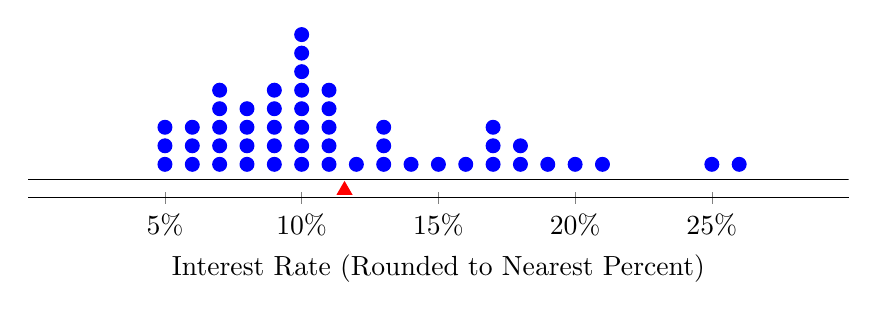
\begin{tikzpicture}
\pgfplotsset{ every non boxed x axis/.append style={x axis line style=-},
     every non boxed y axis/.append style={y axis line style=-}}
\begin{axis}[
width=12cm,
height=3.7cm,
xlabel={Interest Rate (Rounded to Nearest Percent)},
ylabel={},
yticklabels={},
axis y line=none,
axis x line=bottom,
xticklabel=\pgfmathprintnumber{\tick}\%,
xtick={5,10,15,20,25},
ymin=0,
ymax=9,
xmin=0,
xmax=30,
scatter/use mapped color={
 %draw=mapped color,
 fill=blue,
},
]
\addplot [domain=0:30]  {1};
\addplot[scatter, only marks, blue, scatter src=y, mark size=2.5pt]
coordinates
{
(11, 1.8)
(11, 2.8)
(11, 3.8)
(11, 4.8)
(11, 5.8)
(10, 1.8)
(10, 2.8)
(10, 3.8)
(10, 4.8)
(10, 5.8)
(10, 6.8)
(10, 7.8)
(10, 8.8)
(26, 1.8)
(9, 1.8)
(9, 2.8)
(9, 3.8)
(9, 4.8)
(9, 5.8)
(17, 1.8)
(17, 2.8)
(17, 3.8)
(6, 1.8)
(6, 2.8)
(6, 3.8)
(8, 1.8)
(8, 2.8)
(8, 3.8)
(8, 4.8)
(13, 1.8)
(13, 2.8)
(13, 3.8)
(5, 1.8)
(5, 2.8)
(5, 3.8)
(7, 1.8)
(7, 2.8)
(7, 3.8)
(7, 4.8)
(7, 5.8)
(25, 1.8)
(18, 1.8)
(18, 2.8)
(19, 1.8)
(14, 1.8)
(20, 1.8)
(15, 1.8)
(12, 1.8)
(16, 1.8)
(21, 1.8)
};
\addplot [scatter, only marks, red, scatter src=y, mark size=3pt, scatter/use mapped color={fill=red,}, mark=triangle*] coordinates {(11.567, 0.4)};
\end{axis}
\end{tikzpicture}
\end{center}
\end{example}
\end{frame}

\begin{frame}
\begin{definition}
The \textbf{median} of a data set is the measure of center that is the middle value when the original data values are arranged in order of increasing magnitude.
\end{definition}\pause

\begin{block}{Properties}
\begin{itemize}
\item The median does not change by large amounts when we include just a few extreme value. (The median is resistant.)\pause
\item The median does not directly use every data value.
\end{itemize}
\end{block}\pause

\begin{block}{Notation}
The median of a sample is denoted $\tilde{x}$.
\end{block}\pause

\begin{block}{Procedure}
\begin{enumerate}
\item Sort the values.
\item 
\begin{itemize}
\item If the number of data values is odd, the median is the number located in the exact middle of the sorted list.
\item If the number of data values is even, the median is found by computing the mean of the two middle numbers in the sorted list.
\end{itemize}
\end{enumerate}
\end{block}
\end{frame}

\begin{frame}
\begin{example}
Data set 32 \textquote{Airport Data Speeds} in Appendix B includes measures of data speeds of smartphones from four different carriers. The table contains five data speeds, in megabits per second (Mbps), for Verizon.

\begin{center}
\begin{tabular}{|ccccc|}\hline
38.5 & 55.6 & 22.4 & 14.1 & 23.1\\\hline
\end{tabular}
\end{center}\pause

First sort the data values.
\begin{center}
\begin{tabular}{|ccccc|}\hline
14.1 & 22.4 & \textcolor<3->{blue}{23.1} & 38.5 & 55.6\\\hline
\end{tabular}
\end{center}\pause

We have 5 data values so the median is \textcolor{blue}{23.1} Mbps.
\end{example}\pause

\begin{block}{Note}
This different than the mean 30.74 Mbps.
\end{block}
\end{frame}

\begin{frame}
\begin{example}
Data set 32 \textquote{Airport Data Speeds} in Appendix B includes measures of data speeds of smartphones from four different carriers. The table contains six data speeds, in megabits per second (Mbps), for Verizon.

\begin{center}
\begin{tabular}{|cccccc|}\hline
38.5 & 55.6 & 22.4 & 14.1 & 23.1 & 24.5\\\hline
\end{tabular}
\end{center}\pause

First sort the data values.
\begin{center}
\begin{tabular}{|cccccc|}\hline
14.1 & 22.4 & \textcolor<3->{blue}{23.1} & \textcolor<3->{blue}{24.5} & 38.5 & 55.6\\\hline
\end{tabular}
\end{center}\pause

We have 6 data values so the median is $\dfrac{\textcolor{blue}{23.1}+\textcolor{blue}{24.5}}{2}=23.80$ Mbps.
\end{example}
\end{frame}
\end{document}
